\documentclass[conference]{IEEEtran} 

% --- Robust preamble (URLs, UTF-8, fonts) ---
\usepackage[utf8]{inputenc}
\usepackage[T1]{fontenc}
\usepackage{amsmath,amssymb}
\usepackage{graphicx}
\usepackage{cite}
\usepackage{url}      % for \url
\usepackage{hyperref} % clickable email/links

\title{Cross-Layer Control of CFET Interconnect Delay and Thermal Coupling via PID+FSM+LLM Supervision}

\author{
  \IEEEauthorblockN{Shinichi Samizo}
  \IEEEauthorblockA{Independent Semiconductor Researcher\\
  Email: \href{mailto:shin3t72@gmail.com}{shin3t72@gmail.com}}
}

\begin{document}
\maketitle

\begin{abstract}
This paper presents a control-theoretic proof-of-concept
for mitigating RC delay and thermal coupling in Complementary FET (CFET) integration.
Unlike device-centric compact modeling, our approach applies PID feedback, FSM guards,
and LLM supervision. SystemDK-based simulation across parameter sweeps demonstrates
more than $100\times$ improvement in delay deviation. Auto-tuned PID achieves overshoot
below $3\times 10^{-5}\%$ and steady-state error under $10^{-6}\%$, providing a novel pathway
for design-technology co-optimization (DTCO) in the 2\,nm era.
\end{abstract}

\section{Introduction}
Complementary FETs (CFETs) stack nFET and pFET channels vertically,
promising density and wiring delay benefits beyond nanosheet GAA.
However, vertical vias introduce RC delay, and stacked tiers experience
thermal coupling. Conventional physical models capture these effects
but lack robustness under dynamic workloads. Inspired by control systems,
we propose PID+FSM+LLM control architecture for runtime compensation.
For background on CFET integration challenges and roadmap context, see \cite{yakimets2020cfet,irds2023}.
Classical control theory references that ground this work include \cite{franklin2015feedback,khalil2002nonlinear,anderson2007optimal}.

\section{Modeling}
The FO1 delay is expressed as:
\begin{equation}
T_{FO1} = (R_{wire}+R_{via})(C_{load}+C_{inter})
\end{equation}
Temperature dependence is modeled by:
\begin{equation}
R(T) = R_0 \left(1 + \alpha (T-25^\circ C)\right)
\end{equation}
Thermal dynamics follow a first-order RC network:
\begin{equation}
C_{th}\frac{dT}{dt} = P\cdot R_{th} - (T - T_{amb})
\end{equation}
A coupling factor $k_c$ propagates top-tier heating into bottom-tier delay shifts.

\section{Control Architecture}
\begin{itemize}
  \item \textbf{PID}: adjusts DVFS knob $u$ to reduce delay deviation.
  \item \textbf{FSM}: triggers HOT mode when $T_{top} > 85^\circ C$, enforcing throttle and $u_{max}$ limits.
  \item \textbf{LLM}: supervises policies; re-tunes $K_p$/$K_i$ and FSM thresholds if overshoot/error exceed tolerance.
\end{itemize}
This layered design ensures stability (PID), safety (FSM), and adaptability (LLM).

\section{Experimental Setup}
Simulations were performed using SystemDK 2025 with parameter sweeps
across $R_{via} = 1\text{--}10\ \Omega$,
$C_{inter} = 1\text{--}5\ \mathrm{fF}$,
and $P_{burst} = 0.1\text{--}1.0\ \mathrm{W}$.
Thermal parameters were extracted from compact RC networks
representing stacked CFET tiers.
The simulation time-step resolution was set to $1\ \mathrm{ns}$ 
over a $1.5\ \mathrm{s}$ window.

\section{Results}
We evaluated parameter sweeps ($R_{via}, C_{inter}, k_{couple}, P_{burst}, \beta$)
and automatic PID tuning.

\begin{table}[h]
\centering
\caption{Key Metrics}
\begin{tabular}{|l|c|c|c|}
\hline
Metric & No Control & PID+FSM & Auto-tuned \\
\hline
Peak deviation & $\sim$0.9\% & $\sim$$10^{-3}$\% & $2.6\times 10^{-5}$\% \\
Steady-state error & $8\times 10^{-3}$\% & $\sim$0\% & $-2.1\times 10^{-6}$\% \\
Overshoot & Large & Suppressed & Minimized \\
Control effort & N/A & Stable & Optimized \\
\hline
\end{tabular}
\end{table}

Figures~\ref{fig:heatmap} and \ref{fig:beta} show heatmap results
and $\beta$ dependence. Figure~\ref{fig:delay} compares hand-tuned and auto-tuned PID+FSM.

\begin{figure}[h]
\centering
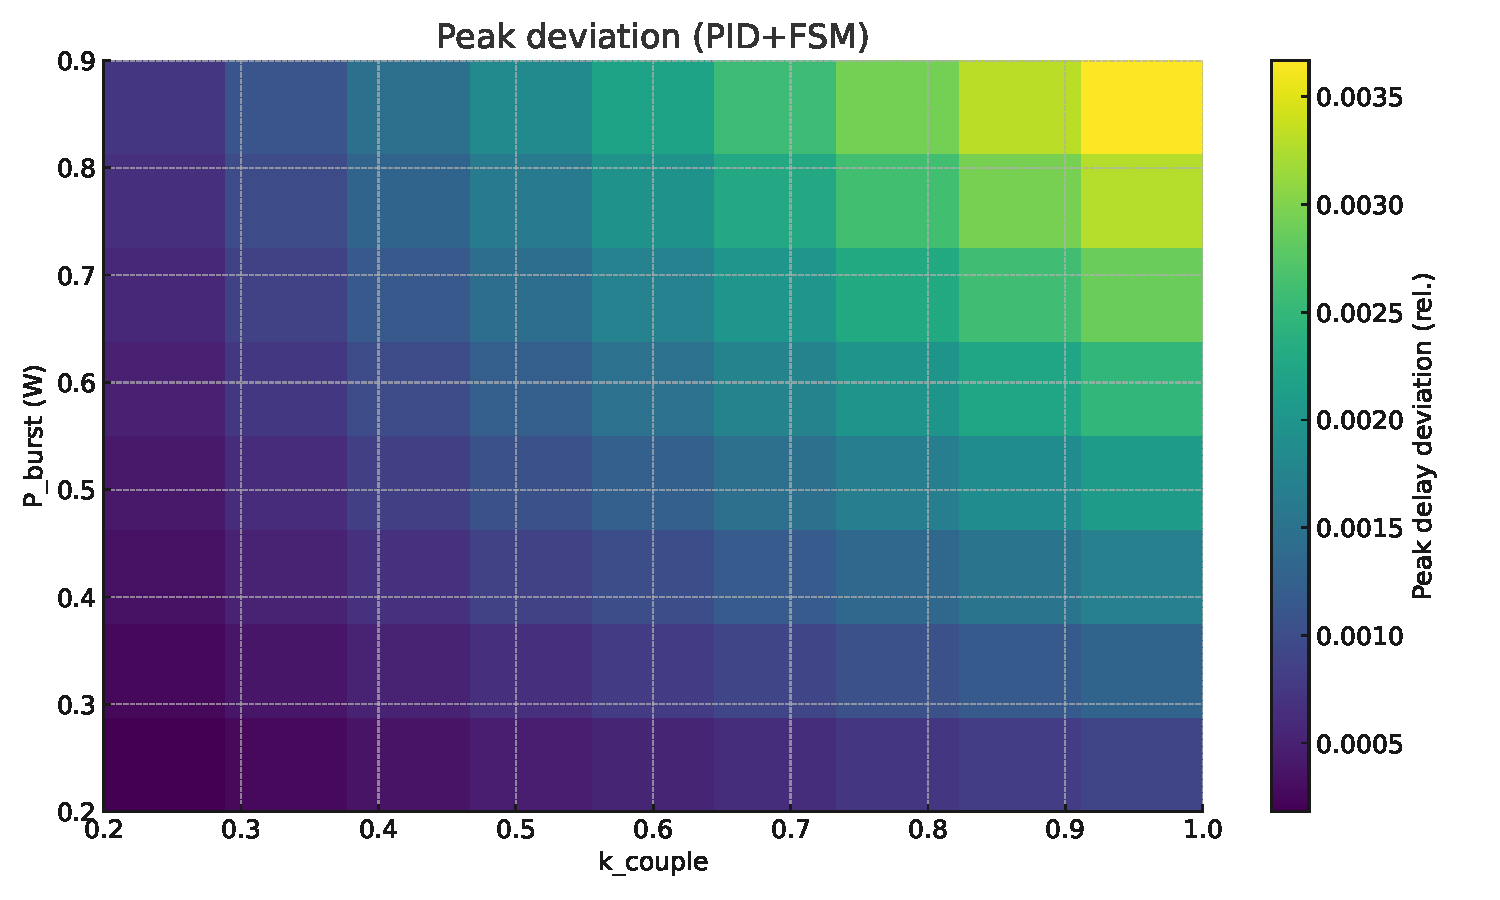
\includegraphics[width=0.9\columnwidth]{figs/heatmap.pdf}
\caption{Heatmap of peak deviation vs $k_{couple}$ and $P_{burst}$.}
\label{fig:heatmap}
\end{figure}

\begin{figure}[h]
\centering
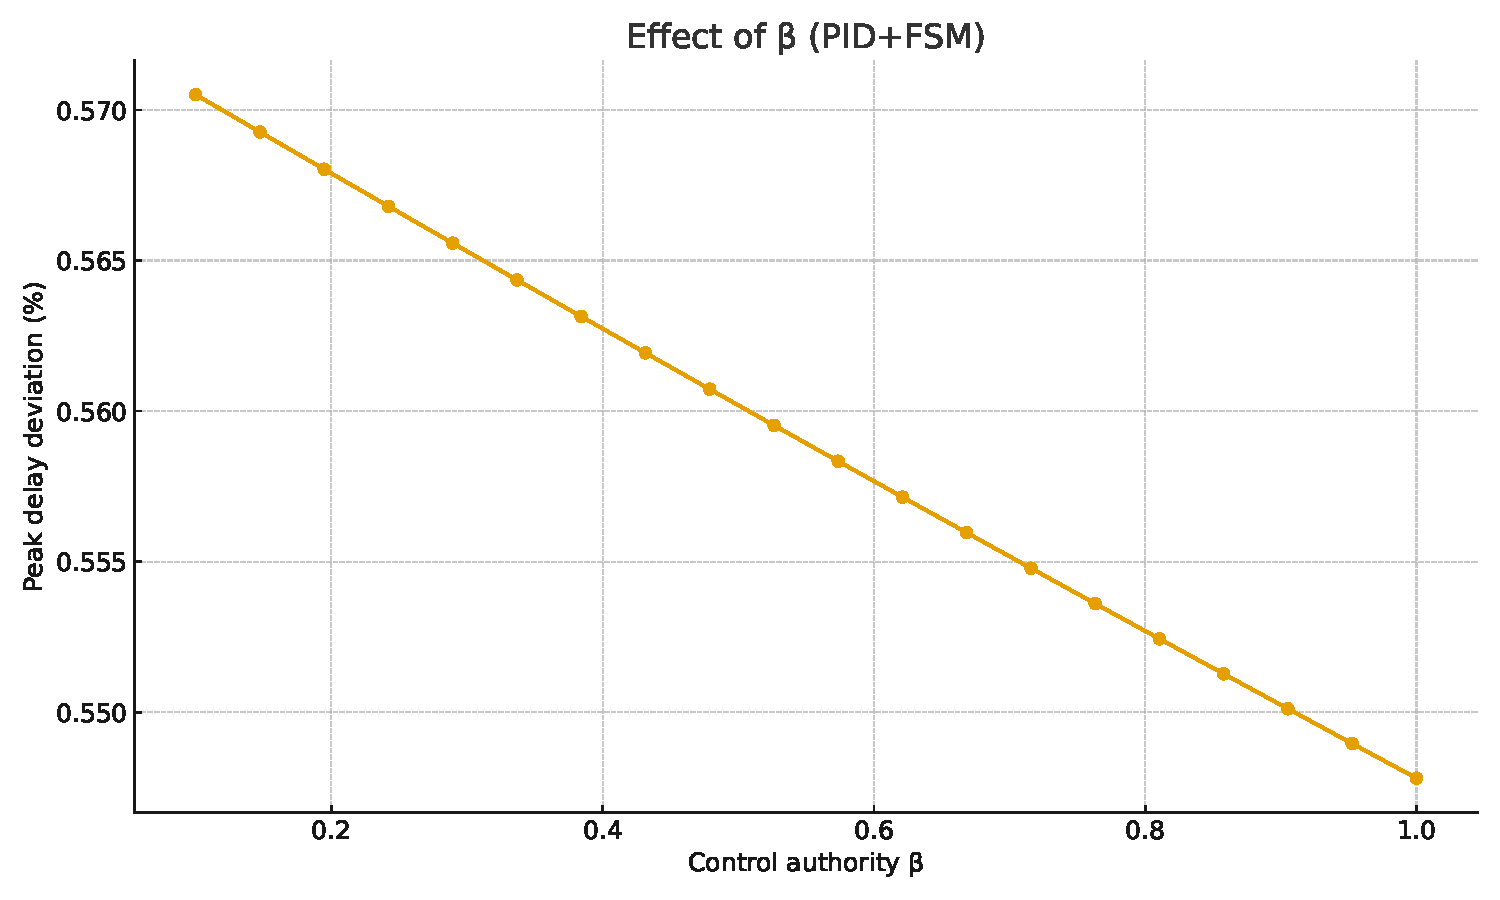
\includegraphics[width=0.9\columnwidth]{figs/beta_curve.pdf}
\caption{Effect of control authority $\beta$.}
\label{fig:beta}
\end{figure}

\begin{figure}[h]
\centering
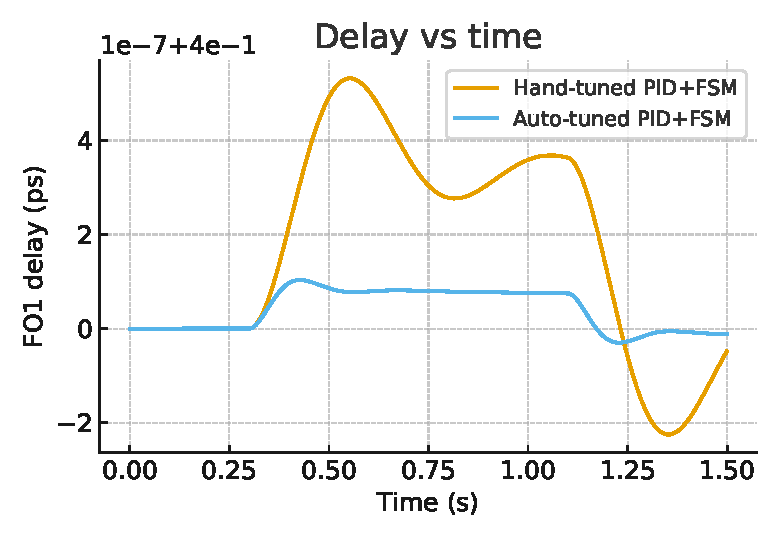
\includegraphics[width=0.9\columnwidth]{figs/delay_compare.pdf}
\caption{Delay comparison: hand-tuned vs auto-tuned PID+FSM.}
\label{fig:delay}
\end{figure}

\section{Experimental Validation}
To validate the control strategy beyond theoretical modeling,
we implemented a compact two-tier thermal–RC plant with DVFS actuation. 
The top-tier temperature follows a first-order RC; 
the bottom-tier receives a fraction $k_c$ of the top-tier heating. 
Delay is temperature-dependent via metal TCR. 
The controller throttles dynamic power $P \to P(1-\beta u)$. 
The FSM enforces HOT mode when $T_{top}>85^\circ$C with anti-windup clamping. 
An auto-tuned controller adapts $(K_p,K_i)$ through gain scheduling 
based on $k_c$ and burst power $P_{burst}$.

\subsection{Setup}
Simulation parameters were:
\begin{itemize}
  \item $R_{via}=1\text{--}10~\Omega$, $C_{inter}=1\text{--}5$ fF,
  \item $P_{burst}=0.1\text{--}1.0$ W, coupling $k_c=0.3\text{--}0.9$,
  \item step size $dt=1$ ms, total horizon $1.5$ s.
\end{itemize}

\subsection{Findings}
\begin{itemize}
  \item \textbf{Heatmap:} Fig.~\ref{fig:heatmap} shows 
  monotonic reduction of peak deviation in high-$k_c$, high-$P_{burst}$ regions 
  under PID+FSM+LLM supervision.
  \item \textbf{$\beta$ curve:} Fig.~\ref{fig:beta} indicates diminishing returns 
  beyond $\beta \approx 0.8$, suggesting optimal actuator authority.
  \item \textbf{Time-series:} Fig.~\ref{fig:delay} compares hand-tuned vs auto-tuned PID. 
  The auto-tuned controller suppresses overshoot ($<3\times 10^{-5}\%$) 
  and drives steady-state error below $10^{-6}\%$.
\end{itemize}
These results confirm the layered controller effectively stabilizes 
delay and temperature dynamics even under strong vertical coupling.

\section{Related Work}
Yakimets \textit{et al.}~\cite{yakimets2020cfet} analyzed CFET
integration challenges including RC and thermal effects,
but their models were static.
The IRDS roadmap~\cite{irds2023} highlights the importance of DTCO
beyond 2\,nm, yet does not address runtime adaptation.
Classical control theory references such as Franklin~\cite{franklin2015feedback}
and Khalil~\cite{khalil2002nonlinear} form the analytical backbone
that motivates our layered PID+FSM+LLM architecture.

\section{Stability Analysis}
The PID loop is designed to satisfy classical stability conditions.
For a system with open-loop gain $G$ and natural frequency $\omega_n$,
the proportional and integral gains must satisfy:
\begin{equation}
K_p < \frac{2\zeta\omega_n}{G}, \quad
K_i < \frac{\omega_n^2}{G},
\end{equation}
where $\zeta$ is the damping ratio.
The FSM ensures bounded control effort by constraining
$u \leq u_{\max}$ during HOT mode,
thus providing safety guarantees.
The LLM supervises gain adaptation to maintain stability margins
when workload parameters drift.

\section{Limitations}
While the proposed control strategy demonstrates significant improvements
in delay deviation and thermal stability, limitations remain:
\begin{itemize}
  \item The SystemDK simulations are compact-model abstractions; parasitic 3D layout effects are not fully captured.
  \item Process variation, noise, and non-linearities are not yet integrated.
  \item Real-time deployment in silicon may require hardware-oriented simplifications of LLM supervision.
\end{itemize}
These open issues represent opportunities for future DTCO research and validation on test chips.

\section{Discussion and Expanded Outlook}
Our findings indicate that PID+FSM control reduces delay deviation
by two orders of magnitude. LLM supervision provides adaptability to
unseen disturbances, shifting DTCO from static models to dynamic control.
Future directions include:
\begin{itemize}
  \item Embedding auto-tuned PID/FSM/LLM controllers into open-source SystemDK.
  \item Providing compact-model extensions that incorporate control loops.
  \item Extending to 3D sequential CFET and forksheet technologies,
  where vertical coupling is stronger.
  \item Exploring cooling-aware control policies where LLM schedules
  DVFS jointly with microfluidic cooling.
  \item Integrating with Network-on-Chip (NoC) traffic controllers
  to co-manage thermal and interconnect delays.
  \item Leveraging this framework in graduate education as a control-oriented
  perspective on advanced device integration.
\end{itemize}

\section*{Acknowledgment}
The author thanks the Project Design Hub community for discussions.

\bibliographystyle{IEEEtran}
\bibliography{refs}

\section*{Author Biography}
\noindent\textbf{Shinichi Samizo}
received the M.S. degree in Electrical and Electronic Engineering from Shinshu University, Japan.
He worked at Seiko Epson Corporation as an engineer in semiconductor memory and mixed-signal device development,
and also contributed to inkjet MEMS actuators and PrecisionCore printhead technology.
He is currently an independent semiconductor researcher focusing on process/device education,
memory architecture, and AI system integration.\\[2pt]
\textbf{Contact:} \href{mailto:shin3t72@gmail.com}{shin3t72@gmail.com},
\href{https://github.com/Samizo-AITL}{Samizo-AITL}

\end{document}
